\chapter{Het p-blok II: zuurstof, halogenen en edelgassen}\label{ch:b1:p-block-16-18}

Van zwavelzuur wordt een grotere tonnage gemaakt dan van welke andere
chemische stof ook: het lost fosfaaterts op voor kunstmest, loogt koper-
en uraniumertsen uit, raffineert olie en vult autobatterijen, en een eeuw
lang was de productie van zwavelzuur een ruwe maat voor de industrie van
een land. Het grootste deel van de zwavel komt nu van de reiniging van
aardgas en olie; een deel wordt nog met de hand uit vulkaankraters
gedragen. Zwavel staat in \omterm{def:b1:periodicity:table}{groep} 16 onder zuurstof; de \omterm{def:b1:p-block-16-18:halogen}{halogenen} van \omterm{def:b1:periodicity:table}{groep}
17 en de edelgassen van \omterm{def:b1:periodicity:table}{groep} 18 vervolledigen het \omterm{def:b1:periodicity:table}{p-blok}. Dit hoofdstuk
volgt zuurstof en zwavel van het element tot het zuur, rangschikt de
\omterm{def:b1:p-block-16-18:halogen}{halogenen} als \omterm{def:b1:nernst:couple}{oxidatoren} met hun \omterm{def:b1:nernst:electrode-potential}{standaardpotentialen}, en eindigt met de
verbindingen die de zogenaamd inerte edelgassen wel degelijk vormen.

\begin{recall}
Lewisstructuren, uitgebreide octetten en de VSEPR-vormen (\cref{ch:b1:lewis-resonance-vsepr});
\omterm{def:b1:nernst:electrode-potential}{standaardpotentialen} (\cref{ch:b1:nernst}); de \omterm{def:b1:e-ph-diagrams:disproportionation}{disproportionering} van
chloor en het \omterm{def:b1:e-ph-diagrams:e-ph-diagram}{potentiaal-pH-diagram} van chloor
(\cref{ch:b1:e-ph-diagrams}); katalyse (\cref{ch:b1:elementary-steps}).
Het schoolboek (jaar 10) groepeerde de \omterm{def:b1:p-block-16-18:halogen}{halogenen} en de edelgassen als
families.
\end{recall}

\begin{omfigure}
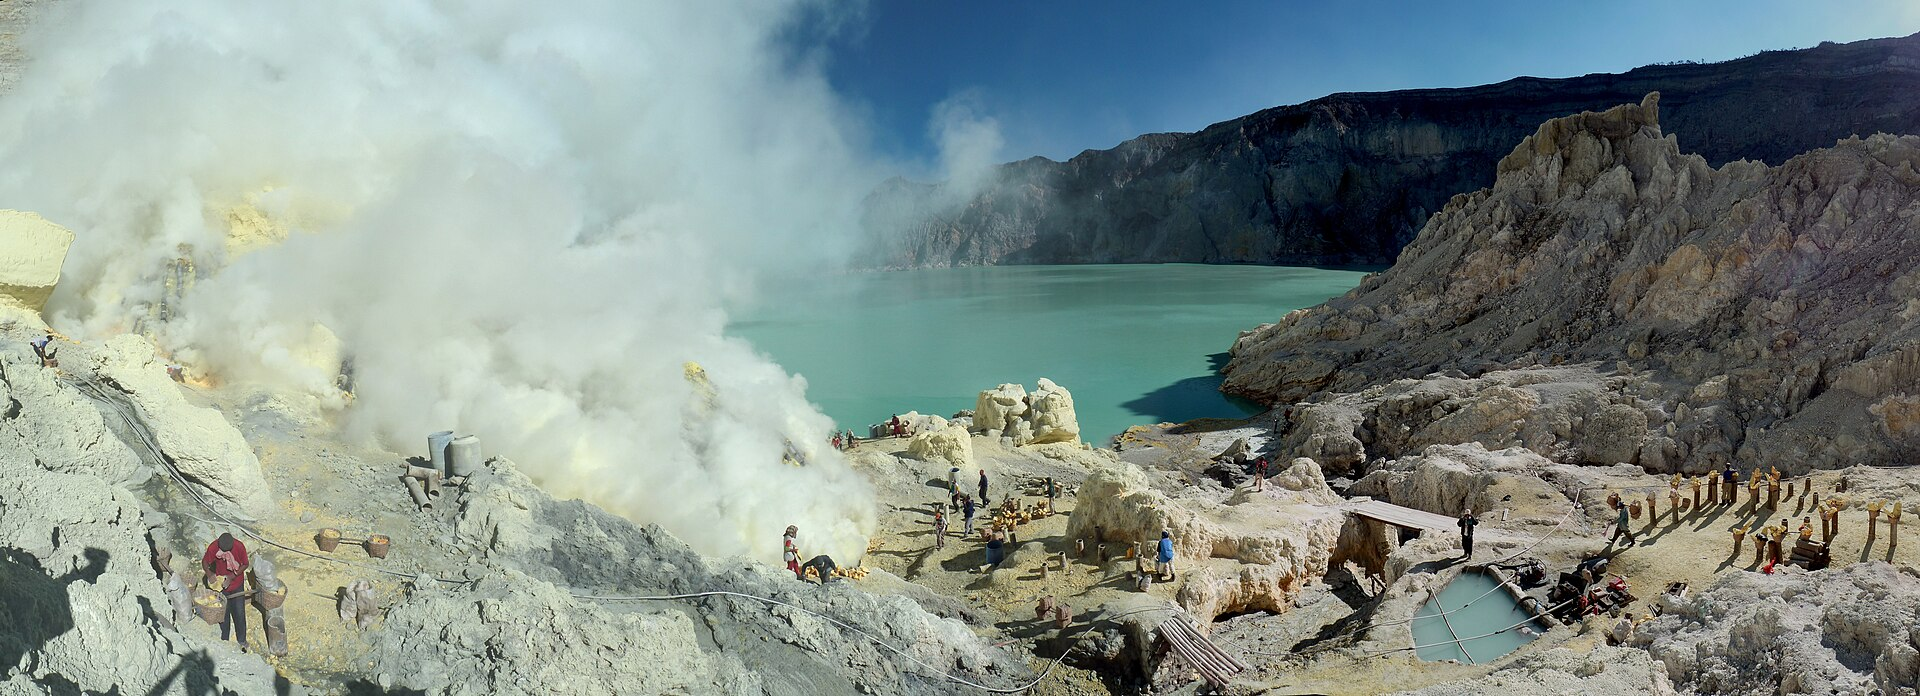
\includegraphics[width=0.78\linewidth]{images/book2/kawah-ijen.jpg}

{\small Zwavelwinning in de krater van de vulkaan Kawah Ijen, Indonesië:
vulkanische gassen condenseren gele zwavel rond buizen, en mijnwerkers
dragen hem in manden naar buiten (foto Sémhur, CC BY-SA 4.0, Wikimedia
Commons).}
\end{omfigure}

\section{Zuurstof, ozon en peroxiden}

\begin{definition}[Chalcogenen]\label{def:b1:p-block-16-18:chalcogen}
De \emph{chalcogenen}\index{chalcogeen} zijn de elementen van \omterm{def:b1:periodicity:table}{groep} 16
(O, S, Se, Te, Po), met zes \omterm{def:b1:quantum-numbers:configuration}{valentie-elektronen} \textit{ns}$^2$\textit{np}$^4$.
Ze vormen verbindingen met \omterm{def:b1:nernst:oxidation-number}{oxidatiegetallen} van $-$II (oxiden, sulfiden)
tot $+$VI (sulfaten), de hogere alleen vanaf zwavel en lager in de groep.
\end{definition}

Zuurstof bestaat als dizuurstof \ce{O2} en als ozon \ce{O3}, een gebogen
molecuul met twee \omterm{def:b1:lewis-resonance-vsepr:resonance}{resonantiestructuren} (\cref{ch:b1:lewis-resonance-vsepr}).
Ozon is een sterkere \omterm{def:b1:nernst:couple}{oxidator} dan dizuurstof: $E^\circ(\ce{O3}/\ce{O2}) = 2.07$~V tegenover 1.23~V voor \ce{O2}/\ce{H2O}. In de hogere atmosfeer
absorbeert het ultraviolet licht; dicht bij de grond is het een
verontreinigende stof. Waterstofperoxide, met een \ce{O-O}-binding en
zuurstof op $-$I, is zowel \omterm{def:b1:nernst:couple}{oxidator} als \omterm{def:b1:nernst:couple}{reductor} en disproportioneert
langzaam (\cref{exo:b1:nernst:12}).
% ledger: dfg:O3_g (E0 computed in figdata/bachelor-1/standard-potentials.py)

\begin{example}[De oxidatiegetallen van zuurstof]
Zuurstof, wat \omterm{def:b1:periodicity:electronegativity}{elektronegativiteit} betreft alleen na fluor, staat in
bijna al zijn verbindingen op $-$II: water, oxiden, hydroxiden, sulfaten.
De uitzonderingen volgen uit de regel dat de gedeelde elektronen naar de
elektronegatievere partner gaan en gelijk verdeeld worden tussen
identieke atomen. In waterstofperoxide \ce{H2O2}, H--O--O--H, neemt elk
zuurstofatoom de elektronen van zijn \ce{O-H}-binding, maar deelt het het
\ce{O-O}-paar: $-$I. In kaliumsuperoxide \ce{KO2} draagt het ion \ce{O2-}
één lading voor twee atomen: gemiddeld $-\frac12$. In zuurstofdifluoride
\ce{OF2} wint fluor beide bindingen en staat zuurstof op $+$II. In
\ce{O2} en \ce{O3} staat het op 0. Alleen de toestand $-$II is stabiel
tegenover water; peroxiden en superoxiden zijn \omterm{def:b1:nernst:couple}{oxidatoren}, en \ce{OF2}
een fluoreringsmiddel.
\end{example}

\section{Zwavel en zwavelzuur}

Zwavel vormt, anders dan zuurstof, ringen en ketens van enkelvoudige
\ce{S-S}-bindingen: gewone zwavel bestaat uit \ce{S8}-ringen. Het
verbrandt tot zwaveldioxide, een gebogen molecuul (hoek O--S--O
\ang{119.5}), dat verder geoxideerd kan worden tot zwaveltrioxide, vlak
trigonaal. Beide zijn \omterm{def:b1:s-block:oxide-character}{zure oxiden}: \ce{SO2} geeft zwaveligzuur
($\mathrm{p}K_a$ 1.77 en 7.22), \ce{SO3} zwavelzuur.
% ledger: geo:SO2.aOSO, dfg:SO2_g, dfg:SO3_g

\begin{proposition}[Stappen van het contactproces]\label{prop:b1:p-block-16-18:contact-steps}
Zwavelzuur wordt in vier stappen uit zwavel gemaakt:
(1) \ce{S + O2 -> SO2}; (2) \ce{2SO2 + O2 <=> 2SO3}, over een \omterm{def:b1:elementary-steps:catalyst}{katalysator}
van vanadium(V)oxide; (3) \ce{SO3 + H2SO4 -> H2S2O7} (oleum), waarbij het
trioxide in geconcentreerd zuur geabsorbeerd wordt; (4) \ce{H2S2O7 + H2O -> 2H2SO4}.
In totaal: \ce{2S + 3O2 + 2H2O -> 2H2SO4}.
\end{proposition}

\begin{proof}
Elke stap is kloppend; tel je $2\times(1)$, (2), $2\times(3)$ en
$2\times(4)$ op, dan vallen \ce{SO2}, \ce{SO3} en \ce{H2S2O7} weg, en de
twee \ce{H2SO4} die in stap 3 verbruikt worden, worden in stap 4
teruggevormd, wat \ce{2S + 3O2 + 2H2O -> 2H2SO4} overlaat. Stap 2 is bij
kamertemperatuur thermodynamisch zeer gunstig ($K = 10^{24.8}$ bij
\qty{25}{\celsius}, uit de vormingsgibbsenergieën) maar uiterst traag: de
\omterm{def:b1:elementary-steps:catalyst}{katalysator}, die alleen warm actief is, laat haar verlopen, en het
compromis tussen snelheid en omzetting wordt in het deel van jaar~2
bestudeerd. \ce{SO3} wordt niet rechtstreeks in water geabsorbeerd, omdat
zijn reactie met waterdamp een fijne nevel van zuurdruppeltjes vormt die
door de absorbers heen gaat.
\end{proof}
% ledger: dfg:SO2_g, dfg:SO3_g

\begin{omfigure}
\begin{tikzpicture}[font=\small, >={Stealth}, box/.style={draw, rounded corners, fill=omDef!8, align=center, minimum height=1.0cm}]
  \node[box] (b) at (0,0) {zwavelbrander\\\ce{S + O2 -> SO2}};
  \node[box] (c) at (4.4,0) {converter, \ce{V2O5}\\katalysatorbedden};
  \node[box] (a) at (8.8,0) {absorptietoren\\\ce{SO3} in \ce{H2SO4}};
  \node[box] (d) at (8.8,-2.2) {verdunning\\\ce{H2S2O7 + H2O}};
  \draw[<-, thick] (b.west) -- ++(-0.8,0) node[left] {lucht, S};
  \draw[->, thick] (b) -- node[above] {\ce{SO2}} (c);
  \draw[->, thick] (c) -- node[above] {\ce{SO3}} (a);
  \draw[->, thick] (a) -- node[right] {oleum} (d);
  \draw[->, thick] (d.west) -- ++(-1.2,0) node[left] {\ce{H2SO4}};
  \draw[->, thick] (d.east) -- ++(0.6,0) |- node[pos=0.25, right] {deels terug} (a.east);
\end{tikzpicture}

{\small Het contactproces: verbranden van zwavel, katalytische oxidatie
van \ce{SO2}, absorptie van \ce{SO3} in geconcentreerd zwavelzuur, en
verdunning van het oleum. Een deel van het zuur wordt naar de absorber
teruggevoerd.}
\end{omfigure}

\begin{proposition}[Sterkte van zwavelzuur]\label{prop:b1:p-block-16-18:sulfuric-strength}
In water is de eerste zuurfunctie van zwavelzuur sterk (volledig), de
tweede zwak: $\mathrm{p}K_a(\ce{HSO4-}/\ce{SO4^2-}) = 1.99$. Een oplossing
van \qty{0.010}{mol/L} heeft daarom geen pH van 1.70 (twee protonen) en
ook geen 2.00 (één), maar een waarde daartussen.
\end{proposition}

\begin{proof}
\ce{H2SO4}, met twee zuurstofatomen zonder waterstof op zwavel, is een
\omterm{def:b1:p-block-13-15:oxoacid}{oxozuur} dat sterker is dan \ce{H3O+}: genivelleerd
(\cref{ch:b1:predominant-reaction}). \ce{HSO4-}, dat al negatief is, houdt
zijn proton steviger vast: zijn $\mathrm{p}K_a$, berekend uit de
vormingsgibbsenergieën, is 1.99. Bij $C = 0.010$:
$[\ce{H3O+}] = C + x$, $[\ce{HSO4-}] = C - x$, $[\ce{SO4^2-}] = x$, met
$x(C + x)/(C - x) = 10^{-1.99}$; oplossen geeft $x = \qty{4.2e-3}{mol/L}$
en $\mathrm{pH} = -\log(0.0142) = 1.85$.
\end{proof}
% ledger: dfg:HSO4-_ao, dfg:SO42-_ao

Geconcentreerd zwavelzuur is ook een krachtig ontwateringsmiddel (het
verkoolt suiker door er de elementen van water aan te onttrekken) en,
heet, een \omterm{def:b1:nernst:couple}{oxidator}. Bij het verdunnen komt veel warmte vrij: het zuur
wordt altijd in het water gegoten, nooit andersom. Het grootste deel van
de zwavel van de wereld, ongeveer 84 miljoen ton in 2025, wordt
teruggewonnen uit het waterstofsulfide van aardgas en van
raffinaderijstromen, en het meeste ervan eindigt als zwavelzuur.
% ledger: usgs:S-world-2025

\begin{method}[Massabalans door het contactproces]\label{met:b1:p-block-16-18:contact-balance}
\begin{enumerate}
  \item Gebruik de totale vergelijking: één \ce{H2SO4} per S-atoom.
  \item Corrigeer voor de omzetting van stap 2 (de fractie \ce{SO2} die
        geoxideerd wordt) en voor de verliezen bij de absorptie.
  \item Voor de lucht: bereken de nodige \ce{O2} (drie halve per S) en
        deel door haar fractie in lucht.
\end{enumerate}
\end{method}

\begin{example}[Een fabriek die duizend ton zwavel per dag verbrandt]
Een fabriek verbrandt \qty{1000}{t} zwavel per dag, zet
\qty{99.0}{\percent} van de \ce{SO2} om en absorbeert
\qty{99.9}{\percent} van de \ce{SO3}. Dan is
$n(\ce{S}) = \num{1000e6}/32.1 = \qty{3.12e7}{mol}$ en
$n(\ce{H2SO4}) = \num{3.12e7} \times 0.990 \times 0.999
= \qty{3.08e7}{mol}$, dus $\num{3.08e7} \times \qty{98.1}{g}
= \qty{3020}{t}$ zuur per dag. De niet-omgezette \qty{1.0}{\percent}
vertrekt als \ce{SO2}: \qty{3.1e5}{mol}, of \qty{20}{t} per dag, die uit
het afgas verwijderd moet worden. De nodige dizuurstof is $1.5 \times \num{3.12e7} =
\qty{4.67e7}{mol}$; lucht, met \qty{21}{\percent} \ce{O2}, is
\qty{2.23e8}{mol}, of $V = nRT/p = \qty{5.5e6}{m^3}$ per dag bij
\qty{25}{\celsius} en \qty{1}{bar}, nog zonder de overmaat die de fabriek
in werkelijkheid inblaast.
\end{example}
% ledger: air:O2

\section{De halogenen}

\begin{definition}[Halogenen]\label{def:b1:p-block-16-18:halogen}
De \emph{halogenen}\index{halogeen} zijn de elementen van \omterm{def:b1:periodicity:table}{groep} 17 (F,
Cl, Br, I, At), met zeven \omterm{def:b1:quantum-numbers:configuration}{valentie-elektronen} \textit{ns}$^2$\textit{np}$^5$.
Ze bestaan als tweeatomige moleculen \ce{X2} en vormen halogenide-ionen
\ce{X-}.
\end{definition}

\begin{omfigure}
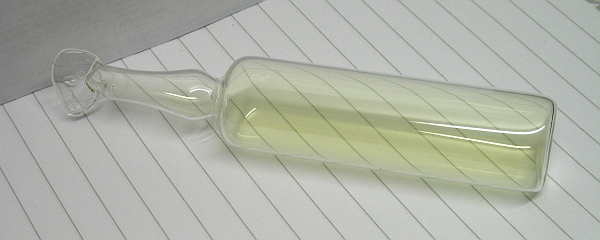
\includegraphics[height=2.9cm]{images/book2/chlorine.jpg}\hspace{0.5em}%
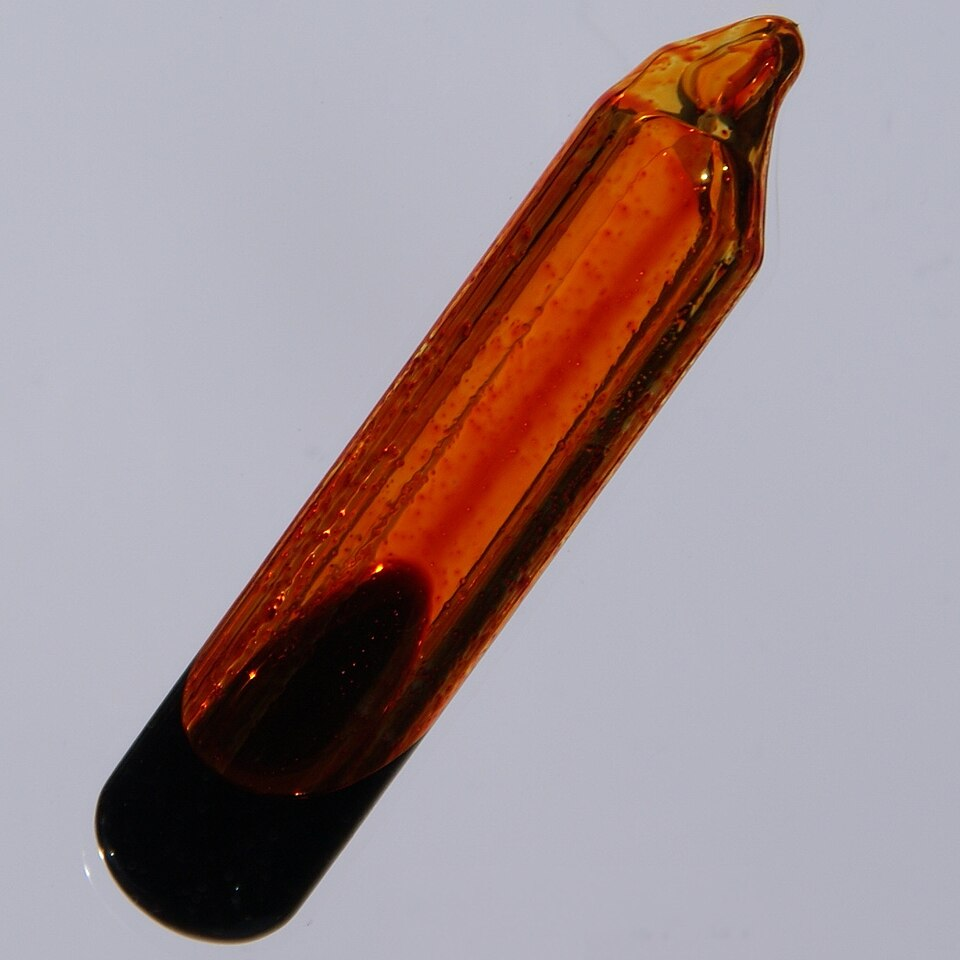
\includegraphics[height=2.9cm]{images/book2/bromine.jpg}\hspace{0.5em}%
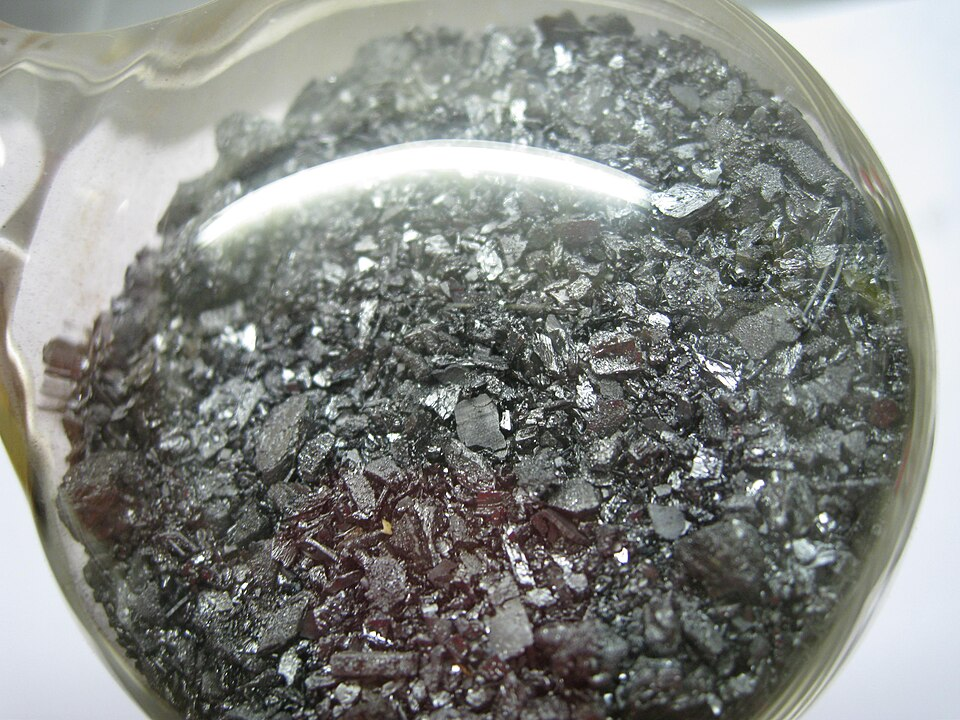
\includegraphics[height=2.9cm]{images/book2/iodine.jpg}

{\small Chloor, een lichtgeelgroen gas (W. Oelen, CC BY-SA 3.0); broom,
een donkerrode vloeistof met een oranje damp (Jurii, CC BY 3.0); jood,
grijszwarte \omterm{def:b1:crystals-metals:crystal}{kristallen} met een metaalglans (Dnn87, CC BY 3.0). Chloor en
broom zijn in glazen ampullen ingesmolten. Alle Wikimedia Commons.}
\end{omfigure}

\begin{proposition}[Oxiderend vermogen van de halogenen]\label{prop:b1:p-block-16-18:halogen-oxidising-order}
De \omterm{def:b1:p-block-16-18:halogen}{halogenen} zijn \omterm{def:b1:nernst:couple}{oxidatoren} waarvan de sterkte naar beneden in de groep
afneemt: $E^\circ(\ce{F2}/\ce{F-}) = 2.89$~V, \ce{Cl2}/\ce{Cl-} 1.36~V,
\ce{Br2}/\ce{Br-} 1.08~V, \ce{I2}/\ce{I-} 0.53~V. Elk \omterm{def:b1:p-block-16-18:halogen}{halogeen} oxideert de
halogenide-ionen die eronder in de groep staan.
\end{proposition}

\begin{proof}
De waarden volgen uit de vormingsgibbsenergieën van de halogenide-ionen
(\cref{ch:b1:nernst}). Volgens de gammaregel oxideert \ce{X2} het ion
\ce{Y-} wanneer het koppel \ce{X2}/\ce{X-} boven \ce{Y2}/\ce{Y-} ligt:
bijvoorbeeld \ce{Cl2 + 2Br- -> 2Cl- + Br2}, $\log K = 2(1.36 - 1.08)/0.059 = 9.5$.
Naar beneden in de groep worden de atomen groter, nemen hun affiniteit
voor een extra elektron en de hydratatie van de kleinere halogenide-ionen
af, en daarmee ook de potentiaal.
\end{proof}
% ledger: dfg:F-_ao, dfg:Cl-_ao, dfg:Br-_ao, dfg:I-_ao

\begin{omfigure}
\begin{tikzpicture}
\begin{axis}[
  ybar, width=0.62\linewidth, height=5.0cm, ymin=0, ymax=3.3,
  symbolic x coords={F,Cl,Br,I}, xtick=data,
  xticklabels={\ce{F2}/\ce{F-}, \ce{Cl2}/\ce{Cl-}, \ce{Br2}/\ce{Br-}, \ce{I2}/\ce{I-}},
  ylabel={$E^\circ$ (V)}, bar width=16pt, nodes near coords,
  every node near coord/.append style={font=\scriptsize},
  tick label style={font=\small}, label style={font=\small}, enlarge x limits=0.2]
\addplot[fill=omThm!40, draw=omThm] coordinates {(F,2.89) (Cl,1.36) (Br,1.08) (I,0.53)};
\end{axis}
\end{tikzpicture}

{\small \omterm{def:b1:nernst:electrode-potential}{Standaardpotentialen} van de koppels halogeen--halogenide bij
\qty{25}{\celsius}, berekend uit getabelleerde gibbsenergieën: het
oxiderend vermogen daalt gestaag naar beneden in de groep.}
\end{omfigure}

De waterstofhalogeniden zijn in water allemaal zuren, maar \ce{HF} is
zwak ($\mathrm{p}K_a$ 3.16) terwijl \ce{HCl}, \ce{HBr} en \ce{HI} sterk
zijn: de \ce{H-F}-binding is zeer sterk en het kleine fluoride-ion wordt in
sterke \omterm{def:b1:intermolecular-forces-solvents:hbond}{waterstofbruggen} vastgehouden. Fluor is het elektronegatiefste
element en de sterkste \omterm{def:b1:nernst:couple}{oxidator} van de tabel; het wordt alleen door
elektrolyse verkregen. De \omterm{def:b1:p-block-13-15:oxoacid}{oxozuren} van chloor --- hypochlorigzuur
\ce{HClO}, chloorzuur \ce{HClO3}, perchloorzuur \ce{HClO4} --- worden
sterker met het aantal zuurstofatomen zonder waterstof, zoals bij alle
\omterm{def:b1:p-block-13-15:oxoacid}{oxozuren} (\cref{def:b1:p-block-13-15:oxoacid}); hun wisselwerking met
chloride en chloor werd in kaart gebracht in \cref{ch:b1:e-ph-diagrams}.
% ledger: dfg:HF_ao, dfg:F-_ao

\begin{omfigure}
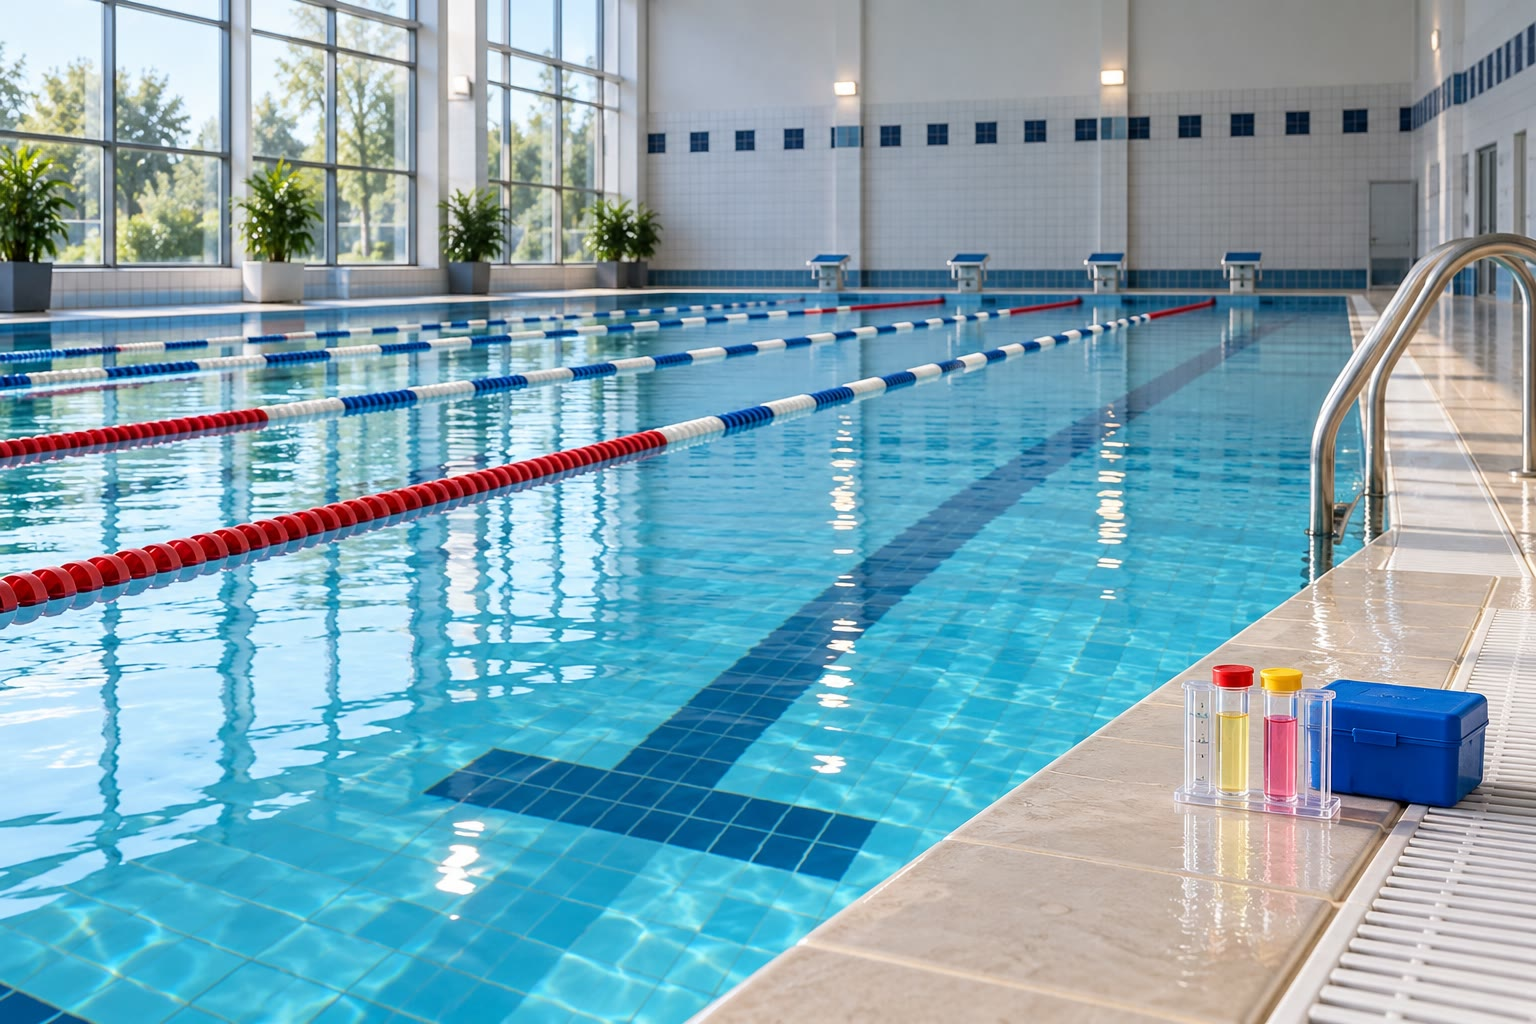
\includegraphics[width=0.55\linewidth]{images/book2/ai/b1-28-swimming-pool.jpg}

{\small Een openbaar zwembad en zijn testset voor het water: het chloor,
opgelost als hypochlorigzuur, wordt meerdere keren per dag gecontroleerd.}
\end{omfigure}

\begin{definition}[Interhalogeenverbindingen]\label{def:b1:p-block-16-18:interhalogen}
Een \emph{interhalogeenverbinding}\index{interhalogeenverbinding} is een
verbinding van twee verschillende \omterm{def:b1:p-block-16-18:halogen}{halogenen}: \ce{ICl}, \ce{BrF3},
\ce{ClF3}, \ce{IF7}. Het grotere, minder elektronegatieve \omterm{def:b1:p-block-16-18:halogen}{halogeen} is het
\omterm{def:b1:complexation:complex}{centrale atoom}, met een uitgebreid octet in \ce{ClF3} en hoger.
\end{definition}

\begin{inthelab}[De halogenen hanteren]
Chloor is giftig en wordt alleen in kleine hoeveelheden in een zuurkast
bereid; broom verbrandt de huid en zijn damp tast de longen aan, en het
wordt verdund gebruikt, in een zuurkast, met handschoenen en
veiligheidsbril, met een oplossing van natriumthiosulfaat bij de hand om
gemorst broom te vernietigen
(\ce{4Br2 + S2O3^2- + 5H2O -> 8Br- + 2SO4^2- + 10H+}). Jood is het mildste
van de drie, maar het vlekt en sublimeert; het wordt in een gesloten fles
bewaard.
\end{inthelab}

\section{Edelgassen en hun verbindingen}

De edelgassen (He, Ne, Ar, Kr, Xe, Rn) hebben gevulde valentieschillen en
de hoogste ionisatie-energieën van hun \omterm{def:b1:periodicity:table}{periode} (\cref{ch:b1:periodicity}).
Lang werden ze inert geacht, maar de zwaardere, waarvan de buitenste
elektronen minder stevig vastgehouden worden, reageren wel met de meest
elektronegatieve elementen: xenon geeft \ce{XeF2}, \ce{XeF4}, \ce{XeF6}
en oxiden. Hun vormen volgen de VSEPR-regels, met \omterm{def:b1:lewis-resonance-vsepr:lewis}{vrije paren} op het
xenon.

\begin{example}[Waarom xenon, en niet argon]
De eerste ionisatie-energieën van de edelgassen dalen naar beneden in de
groep: He 24.59, Ne 21.56, Ar 15.76, Kr 14.00, Xe 12.13, Rn 10.75~eV. Die
van dizuurstof, \ce{O2 -> O2+ + e-}, is 12.07~eV, bijna dezelfde als die
van xenon. Een \omterm{def:b1:nernst:couple}{oxidator} die sterk genoeg is om een elektron van \ce{O2}
weg te nemen en zo het dioxygenylkation \ce{O2+} te geven, zou dus ook
xenon moeten oxideren, maar niet argon, dat zijn elektron 3.7~eV steviger
vasthoudt. Xenon reageert inderdaad met de zeer sterke \omterm{def:b1:nernst:couple}{oxidator}
platinahexafluoride \ce{PtF6}, wat een vaste stof geeft met als totale
samenstelling \ce{XePtF6}, en met fluor zelf, dat de xenonfluoriden van
de tabel hieronder geeft. Radon, dat nog gemakkelijker te ioniseren is,
is te radioactief om er veel chemie mee te doen.
\end{example}
% ledger: ie:He, ie:Ne, ie:Ar, ie:Kr, ie:Xe, ie:Rn, ie:O2, lit:XePtF6

\begin{omfigure}
\begin{tabular}{llll}
\hline
molecuul & elektronenparen op het \omterm{def:b1:complexation:complex}{centrale atoom} & vorm & gemeten hoek \\
\hline
\ce{SO2} & 2 bindende domeinen + 1 \omterm{def:b1:lewis-resonance-vsepr:lewis}{vrij paar} & gebogen & \ang{119.5} \\
\ce{SF6} & 6 bindende & octaëdrisch & \ang{90} \\
\ce{ClF3} & 3 bindende + 2 \omterm{def:b1:lewis-resonance-vsepr:lewis}{vrije paren} & T-vormig & \ang{87.5} \\
\ce{XeF2} & 2 bindende + 3 \omterm{def:b1:lewis-resonance-vsepr:lewis}{vrije paren} & lineair & \ang{180} \\
\ce{XeF4} & 4 bindende + 2 \omterm{def:b1:lewis-resonance-vsepr:lewis}{vrije paren} & vierkant vlak & \ang{90} \\
\hline
\end{tabular}

\smallskip
{\small Vormen van enkele moleculen van het \omterm{def:b1:periodicity:table}{p-blok} met uitgebreide
octetten of \omterm{def:b1:lewis-resonance-vsepr:lewis}{vrije paren} (gemeten hoeken waar beschikbaar). De \omterm{def:b1:lewis-resonance-vsepr:lewis}{vrije paren}
van \ce{XeF2} bezetten de drie equatoriale posities van een trigonale
bipiramide, zodat het molecuul lineair is.}
% ledger: geo:SO2.aOSO, geo:SF6.aFSF, geo:ClF3.aFClF, geo:XeF2.aFXeF
\end{omfigure}

Argon, bijna één procent van de lucht, beschermt reactieve materialen in
laboratoria en bij het lassen; helium, uit aardgas, koelt supergeleidende
magneten, zoals die van NMR-spectrometers (\cref{ch:b1:structure-spectroscopy}).
% ledger: air:Ar

\section{Oefeningen}

\begin{exercise}[$\star$]\label{exo:b1:p-block-16-18:1}
Geef het \omterm{def:b1:nernst:oxidation-number}{oxidatiegetal} van zwavel in \ce{H2S}, \ce{S8}, \ce{SO2},
\ce{SO3^2-}, \ce{SO4^2-}, \ce{S2O3^2-} (gemiddeld) en \ce{H2S2O7}.
\end{exercise}

\begin{exercise}[$\star$]\label{exo:b1:p-block-16-18:2}
Welke van deze reacties verlopen: chloor met kaliumjodide; jood met
natriumbromide; broom met natriumchloride; chloor met natriumbromide?
Schrijf de reacties op die verlopen.
\end{exercise}

\begin{exercise}[$\star$]\label{exo:b1:p-block-16-18:3}
Teken de lewisstructuren van \ce{SO2}, \ce{SO3} en \ce{O3}, met hun
\omterm{def:b1:lewis-resonance-vsepr:resonance}{resonantiestructuren}, en geef hun vorm.
\end{exercise}

\begin{exercise}[$\star$]\label{exo:b1:p-block-16-18:4}
Schrijf de reacties op van \ce{SO2} en \ce{SO3} met water en met
natriumhydroxide.
\end{exercise}

\begin{exercise}[$\star\star$]\label{exo:b1:p-block-16-18:5}
Bereken de pH van fluorwaterstofzuur van \qty{0.10}{mol/L} en vergelijk
met zoutzuur van dezelfde concentratie. Verklaar het verschil.
\end{exercise}

\begin{exercise}[$\star\star$]\label{exo:b1:p-block-16-18:6}
Voorspel met VSEPR de vormen van \ce{BrF5}, \ce{IF7} (zeven \omterm{def:b1:lewis-resonance-vsepr:lewis}{bindende
paren}, pentagonale bipiramide), \ce{ICl4-} en \ce{XeO3}.
\end{exercise}

\begin{exercise}[$\star\star$]\label{exo:b1:p-block-16-18:7}
Bereken de constante van \ce{Cl2 + 2I- -> 2Cl- + I2} en zeg waarom
chloorwater een zetmeel-jodidepapiertje blauw kleurt.
\end{exercise}

\begin{exercise}[$\star\star$]\label{exo:b1:p-block-16-18:8}
Toon aan dat ozon jodide-ionen tot jood kan oxideren en schrijf de
reactie in zuur milieu op. Waarom gebruikt men dit om ozon te meten?
\end{exercise}

\begin{exercise}[$\star\star$]\label{exo:b1:p-block-16-18:9}
Geconcentreerd zwavelzuur verkoolt sacharose, \ce{C12H22O11}. Schrijf de
\omterm{def:b1:alcohol-activation:dehydration}{dehydratatie} tot koolstof op en bereken de massa koolstof uit
\qty{10.0}{g} suiker.
\end{exercise}

\begin{exercise}[$\star\star\star$]\label{exo:b1:p-block-16-18:10}
Bereken de pH van zwavelzuur van \qty{0.10}{mol/L}, rekening houdend met
de tweede zuurfunctie ($\mathrm{p}K_a = 1.99$). Hoeveel voegt de tweede
zuurfunctie toe?
\end{exercise}

\begin{exercise}[$\star\star\star$]\label{exo:b1:p-block-16-18:11}
Verklaar met de potentialen waarom fluor niet bereid kan worden door
fluoride met eender welke chemische \omterm{def:b1:nernst:couple}{oxidator} in water te oxideren, en
waarom het gemaakt moet worden door elektrolyse van een gesmolten
fluoride, niet van een waterige oplossing.
\end{exercise}

\begin{exercise}[$\star\star\star$]\label{exo:b1:p-block-16-18:12}
Jood is slechts weinig oplosbaar in water, maar lost op in een
kaliumjodide-oplossing als het trijodide-ion \ce{I3-}. Bereken met de
gibbsenergieën van \ce{I2(aq)} ($\Delta_f G^\circ = \qty{16.40}{kJ/mol}$),
\ce{I-} ($-51.57$) en \ce{I3-} ($-51.4$) de constante van
\ce{I2 + I- <=> I3-}.
\end{exercise}

\section{Probleem: één ton zwavel}

\begin{problem}[{Weekendprobleem --- het verbranden van zwavel, de
katalytische oxidatie van zwaveldioxide, absorptie en oleum, de tweede
zuurfunctie van zwavelzuur, en de massa zuur die uit één ton zwavel
gemaakt wordt}]
\label{pb:b1:p-block-16-18:1}
Een zwavelzuurfabriek verbrandt zwavel die uit aardgas teruggewonnen is.
Molaire massa's (\unit{g/mol}): S 32.1, \ce{O2} 32.0, \ce{SO2} 64.1,
\ce{SO3} 80.1, \ce{H2SO4} 98.1, \ce{H2O} 18.0; lucht bevat
\qty{21}{\percent} \ce{O2} in volume; $\mathrm{p}K_a(\ce{HSO4-}) = 1.99$;
$R =
\qty{8.314}{J/(K.mol)}$.

\medskip
\noindent\textbf{Deel I --- Zwavel verbranden.}
\begin{enumerate}
  \item Geef het \omterm{def:b1:nernst:oxidation-number}{oxidatiegetal} van S in S, \ce{SO2}, \ce{SO3} en
        \ce{H2SO4}.
  \item Schrijf de verbranding van zwavel op.
  \item Teken de \omterm{def:b1:lewis-resonance-vsepr:lewis}{lewisstructuur} van \ce{SO2} en voorspel zijn vorm.
  \item Bereken de hoeveelheid stof zwavel in één ton.
  \item Bereken het volume lucht (\qty{25}{\celsius}, \qty{1}{bar}) voor
        de verbranding alleen.
  \item Waarom wordt het gas uit de brander afgekoeld voor de converter?
\end{enumerate}

\medskip
\noindent\textbf{Deel II --- Katalytische oxidatie.}
\begin{enumerate}[resume]
  \item Schrijf de oxidatie van \ce{SO2} tot \ce{SO3} op.
  \item Haar constante bij \qty{25}{\celsius} is ongeveer $10^{24.8}$.
        Waarom is er toch een \omterm{def:b1:elementary-steps:catalyst}{katalysator} nodig?
  \item Wat is de rol van vanadium(V)oxide, in de taal van
        \cref{ch:b1:elementary-steps}?
  \item Teken de vorm van \ce{SO3}.
  \item Waarom gebruikt men overmaat lucht?
  \item Welke fractie \ce{SO2} gaat verloren als de omzetting
        \qty{99.7}{\percent} bedraagt?
\end{enumerate}

\medskip
\noindent\textbf{Deel III --- Absorptie.}
\begin{enumerate}[resume]
  \item Schrijf de absorptie van \ce{SO3} in zwavelzuur op.
  \item Waarom wordt \ce{SO3} niet rechtstreeks in water geabsorbeerd?
  \item Schrijf de verdunning van oleum op.
  \item Schrijf de totale vergelijking van het proces op.
  \item Bereken de massa water die per ton zwavel verbruikt wordt.
  \item Waarom moet het zuur in water gegoten worden en nooit andersom?
\end{enumerate}

\medskip
\noindent\textbf{Deel IV --- Het zuur.}
\begin{enumerate}[resume]
  \item Bereken de pH van een oplossing van zwavelzuur van
        \qty{0.050}{mol/L}, rekening houdend met de tweede zuurfunctie.
  \item Bereken de massa zwavelzuur bij een totaalrendement van
        \qty{99.5}{\percent}.
  \item De wereld produceerde in 2025 ongeveer \qty{84}{Mt} zwavel.
        Welke massa zwavelzuur zou die geven als alles omgezet werd?
  \item Geef de massa zwavelzuur die uit één ton zwavel verkregen kan
        worden (volledige omzetting).
\end{enumerate}
\end{problem}
